\documentclass{article}
\usepackage[a4paper,landscape,margin=1.5cm]{geometry}
\usepackage{pgfplots}
\pgfplotsset{compat=1.18}
\pagestyle{empty}
\begin{document}
\section*{\texttt{cnot-order1-vs-eps.tex}}
Order 1: CNOT count vs $\varepsilon$ (merged, measured $r$; solid $n=10$, dashed $n=8$)\par\medskip
% Generated by plsimcount.pfeps -- do not edit; regenerate instead.
% order 1, cnot total (merged, cz) vs eps_trotter, n in [8, 10], measured r, seed 1, t = n
% git_commit=01d3c275ceae2840002bd1aaea68f59b987c4975 git_dirty=False
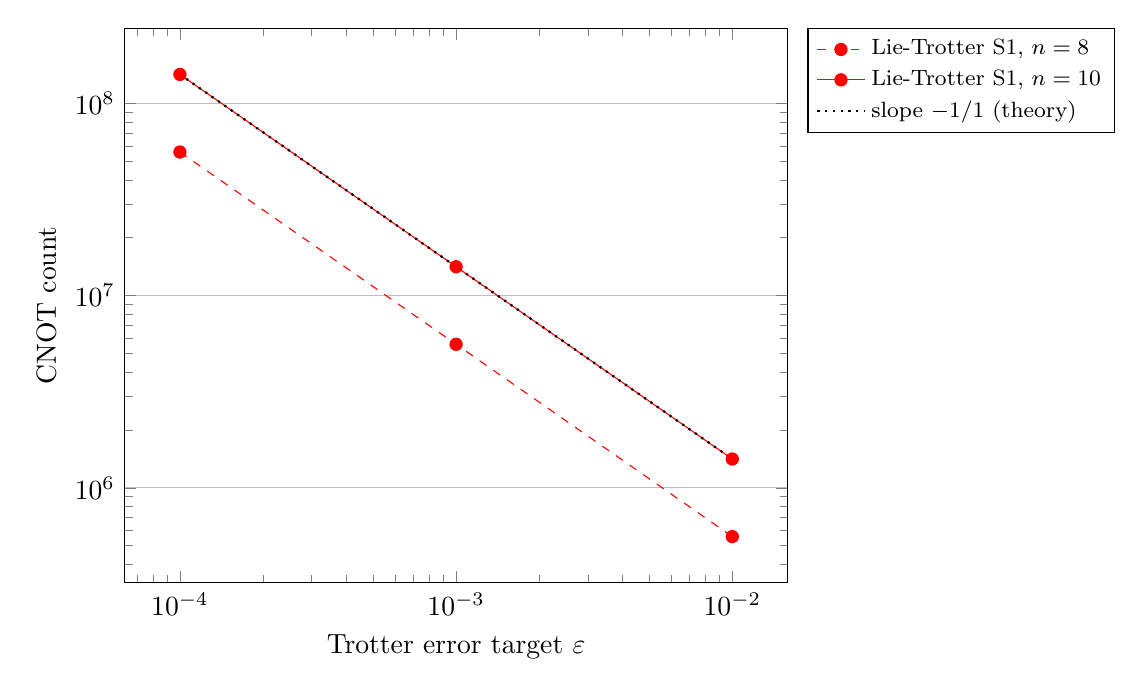
\begin{tikzpicture}
  \begin{loglogaxis}[
    width=10cm,
    xlabel={Trotter error target $\varepsilon$},
    ylabel={CNOT count},
    ymajorgrids=true,
    legend pos=outer north east,
    legend cell align=left,
    legend style={font=\footnotesize},
  ]
    \addplot[red, dashed, mark=*, mark size=2.2pt, mark options={solid, fill=red}] coordinates {
      (0.0001,55785888)
      (0.001,5578704)
      (0.01,558000)
    };
    \addlegendentry{Lie-Trotter S1, $n=8$}
    \addplot[red, solid, mark=*, mark size=2.2pt, mark options={solid, fill=red}] coordinates {
      (0.0001,141274260)
      (0.001,14127480)
      (0.01,1412820)
    };
    \addlegendentry{Lie-Trotter S1, $n=10$}
    \addplot[black, dotted, thick, domain=0.0001:0.01, samples=2] {1.41275e+07*(x/0.001)^(-1)};
    \addlegendentry{slope $-1/1$ (theory)}
  \end{loglogaxis}
\end{tikzpicture}

\clearpage

\section*{\texttt{cnot-order2-vs-eps.tex}}
Order 2: CNOT count vs $\varepsilon$ (merged, measured $r$; solid $n=10$, dashed $n=8$)\par\medskip
% Generated by plsimcount.pfeps -- do not edit; regenerate instead.
% order 2, cnot total (merged, cz) vs eps_trotter, n in [8, 10], measured r, seed 1, t = n
% git_commit=01d3c275ceae2840002bd1aaea68f59b987c4975 git_dirty=False
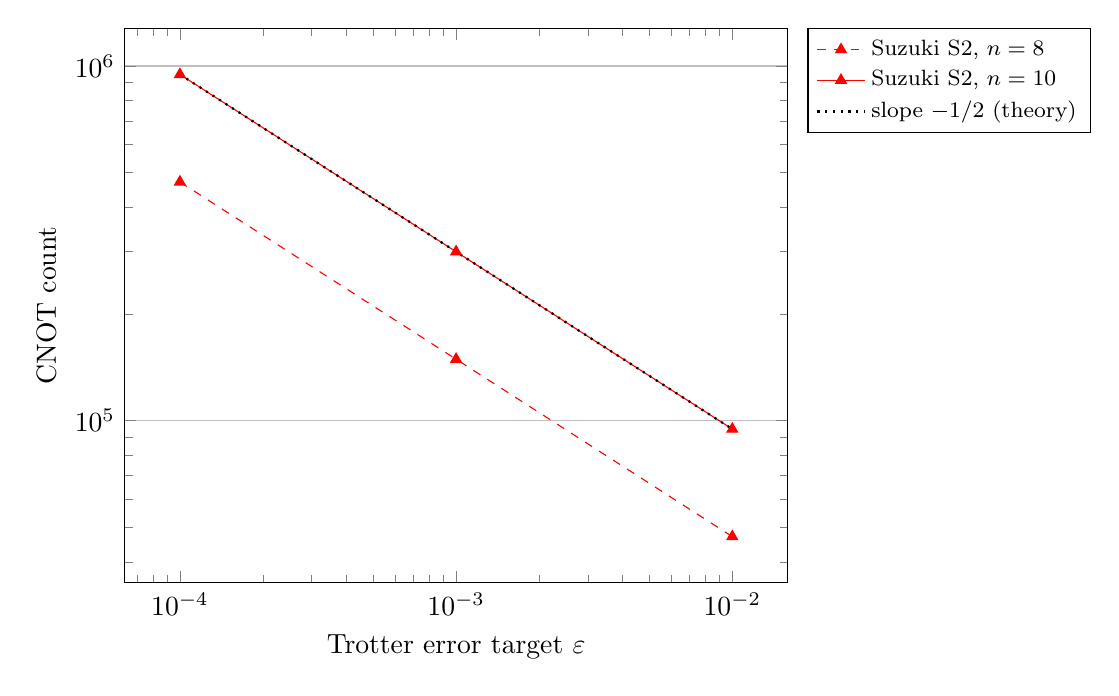
\begin{tikzpicture}
  \begin{loglogaxis}[
    width=10cm,
    xlabel={Trotter error target $\varepsilon$},
    ylabel={CNOT count},
    ymajorgrids=true,
    legend pos=outer north east,
    legend cell align=left,
    legend style={font=\footnotesize},
  ]
    \addplot[red, dashed, mark=triangle*, mark size=2.2pt, mark options={solid, fill=red}] coordinates {
      (0.0001,471120)
      (0.001,149040)
      (0.01,47120)
    };
    \addlegendentry{Suzuki S2, $n=8$}
    \addplot[red, solid, mark=triangle*, mark size=2.2pt, mark options={solid, fill=red}] coordinates {
      (0.0001,946600)
      (0.001,299400)
      (0.01,94700)
    };
    \addlegendentry{Suzuki S2, $n=10$}
    \addplot[black, dotted, thick, domain=0.0001:0.01, samples=2] {299400*(x/0.001)^(-0.5)};
    \addlegendentry{slope $-1/2$ (theory)}
  \end{loglogaxis}
\end{tikzpicture}

\clearpage

\section*{\texttt{cnot-order4-vs-eps.tex}}
Order 4: CNOT count vs $\varepsilon$ (merged, measured $r$; solid $n=10$, dashed $n=8$)\par\medskip
% Generated by pysimcount.pfeps -- do not edit; regenerate instead.
% order 4, cnot total (merged, cz) vs eps_trotter, n in [8, 10], measured r, seed 1, t = n
% git_commit=01d3c275ceae2840002bd1aaea68f59b987c4975 git_dirty=False
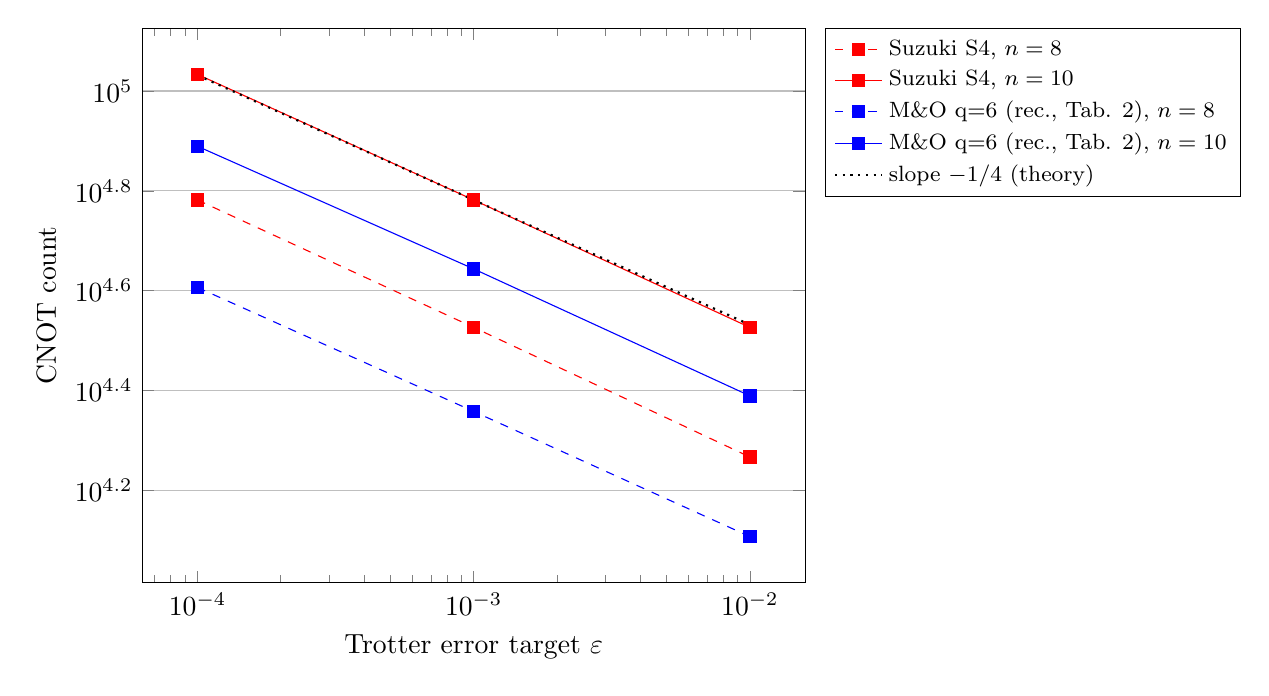
\begin{tikzpicture}
  \begin{loglogaxis}[
    width=10cm,
    xlabel={Trotter error target $\varepsilon$},
    ylabel={CNOT count},
    ymajorgrids=true,
    legend pos=outer north east,
    legend cell align=left,
    legend style={font=\footnotesize},
  ]
    \addplot[red, dashed, mark=square*, mark size=2.2pt, mark options={solid, fill=red}] coordinates {
      (0.0001,60480)
      (0.001,33600)
      (0.01,18480)
    };
    \addlegendentry{Suzuki S4, $n=8$}
    \addplot[red, solid, mark=square*, mark size=2.2pt, mark options={solid, fill=red}] coordinates {
      (0.0001,107940)
      (0.001,60480)
      (0.01,33600)
    };
    \addlegendentry{Suzuki S4, $n=10$}
    \addplot[blue, dashed, mark=square*, mark size=2.2pt, mark options={solid, fill=blue}] coordinates {
      (0.0001,40400)
      (0.001,22800)
      (0.01,12800)
    };
    \addlegendentry{M\&O q=6 (rec., Tab. 2), $n=8$}
    \addplot[blue, solid, mark=square*, mark size=2.2pt, mark options={solid, fill=blue}] coordinates {
      (0.0001,77500)
      (0.001,44000)
      (0.01,24500)
    };
    \addlegendentry{M\&O q=6 (rec., Tab. 2), $n=10$}
    \addplot[black, dotted, thick, domain=0.0001:0.01, samples=2] {60480*(x/0.001)^(-0.25)};
    \addlegendentry{slope $-1/4$ (theory)}
  \end{loglogaxis}
\end{tikzpicture}

\clearpage

\section*{\texttt{cnot-order6-vs-eps.tex}}
Order 6: CNOT count vs $\varepsilon$ (merged, measured $r$; solid $n=10$, dashed $n=8$)\par\medskip
% Generated by pysimcount.pfeps -- do not edit; regenerate instead.
% order 6, cnot total (merged, cz) vs eps_trotter, n in [8, 10], measured r, seed 1, t = n
% git_commit=01d3c275ceae2840002bd1aaea68f59b987c4975 git_dirty=False
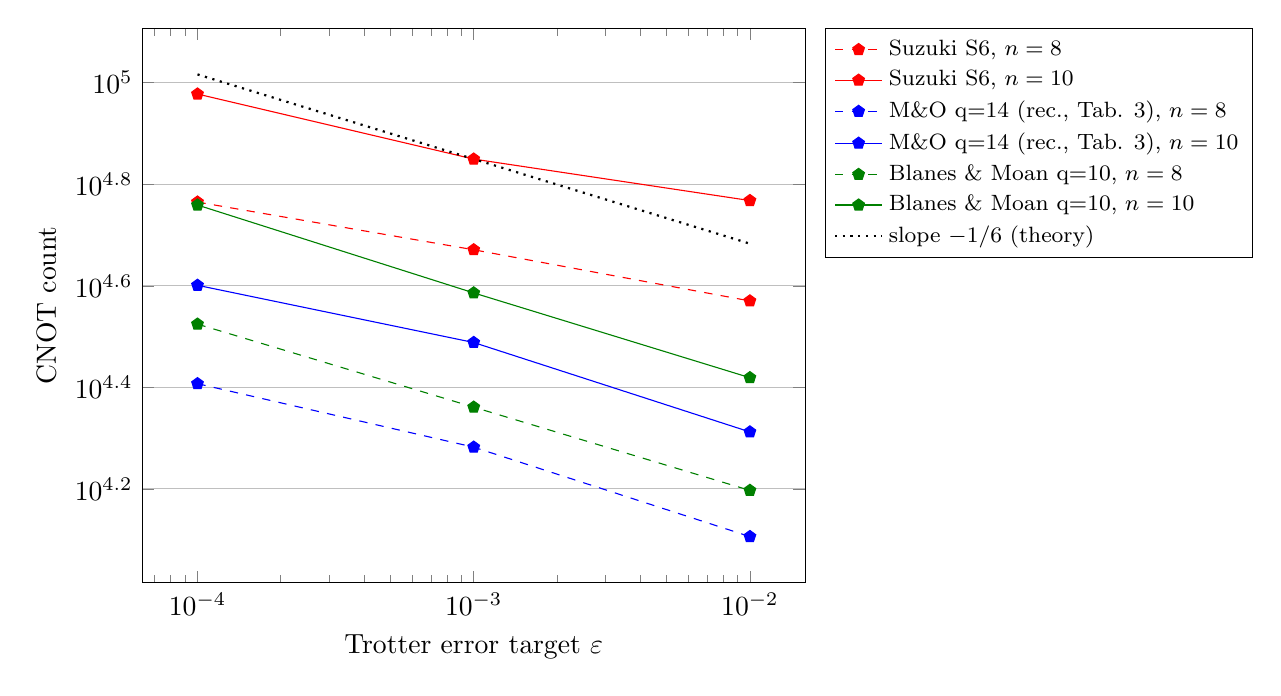
\begin{tikzpicture}
  \begin{loglogaxis}[
    width=10cm,
    xlabel={Trotter error target $\varepsilon$},
    ylabel={CNOT count},
    ymajorgrids=true,
    legend pos=outer north east,
    legend cell align=left,
    legend style={font=\footnotesize},
  ]
    \addplot[red, dashed, mark=pentagon*, mark size=2.2pt, mark options={solid, fill=red}] coordinates {
      (0.0001,58176)
      (0.001,46864)
      (0.01,37168)
    };
    \addlegendentry{Suzuki S6, $n=8$}
    \addplot[red, solid, mark=pentagon*, mark size=2.2pt, mark options={solid, fill=red}] coordinates {
      (0.0001,94940)
      (0.001,70700)
      (0.01,58580)
    };
    \addlegendentry{Suzuki S6, $n=10$}
    \addplot[blue, dashed, mark=pentagon*, mark size=2.2pt, mark options={solid, fill=blue}] coordinates {
      (0.0001,25536)
      (0.001,19152)
      (0.01,12768)
    };
    \addlegendentry{M\&O q=14 (rec., Tab. 3), $n=8$}
    \addplot[blue, solid, mark=pentagon*, mark size=2.2pt, mark options={solid, fill=blue}] coordinates {
      (0.0001,39900)
      (0.001,30780)
      (0.01,20520)
    };
    \addlegendentry{M\&O q=14 (rec., Tab. 3), $n=10$}
    \addplot[green!50!black, dashed, mark=pentagon*, mark size=2.2pt, mark options={solid, fill=green!50!black}] coordinates {
      (0.0001,33456)
      (0.001,22960)
      (0.01,15744)
    };
    \addlegendentry{Blanes \& Moan q=10, $n=8$}
    \addplot[green!50!black, solid, mark=pentagon*, mark size=2.2pt, mark options={solid, fill=green!50!black}] coordinates {
      (0.0001,57400)
      (0.001,38540)
      (0.01,26240)
    };
    \addlegendentry{Blanes \& Moan q=10, $n=10$}
    \addplot[black, dotted, thick, domain=0.0001:0.01, samples=2] {70700*(x/0.001)^(-0.166667)};
    \addlegendentry{slope $-1/6$ (theory)}
  \end{loglogaxis}
\end{tikzpicture}

\clearpage

\section*{\texttt{cnot-order8-vs-eps.tex}}
Order 8: CNOT count vs $\varepsilon$ (merged, measured $r$; solid $n=10$, dashed $n=8$)\par\medskip
% Generated by plsimcount.pfeps -- do not edit; regenerate instead.
% order 8, cnot total (merged, cz) vs eps_trotter, n in [8, 10], measured r, seed 1, t = n
% git_commit=01d3c275ceae2840002bd1aaea68f59b987c4975 git_dirty=False
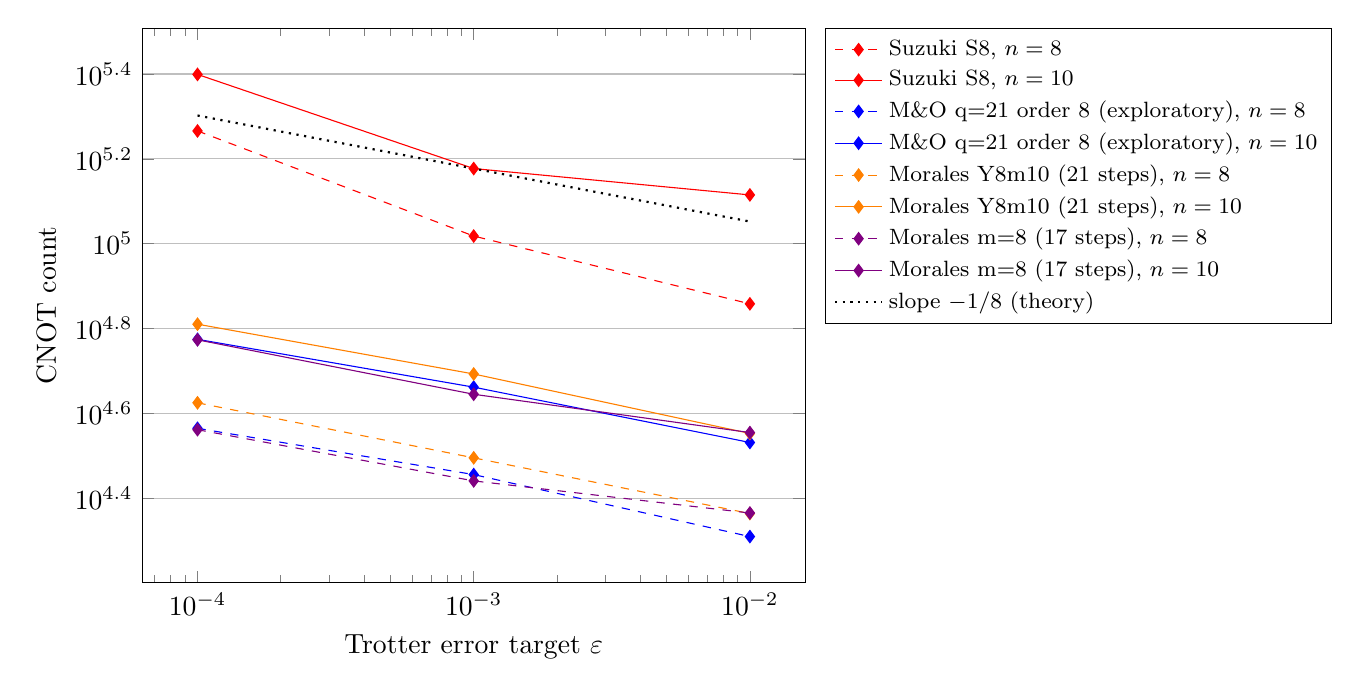
\begin{tikzpicture}
  \begin{loglogaxis}[
    width=10cm,
    xlabel={Trotter error target $\varepsilon$},
    ylabel={CNOT count},
    ymajorgrids=true,
    legend pos=outer north east,
    legend cell align=left,
    legend style={font=\footnotesize},
  ]
    \addplot[red, dashed, mark=diamond*, mark size=2.2pt, mark options={solid, fill=red}] coordinates {
      (0.0001,184368)
      (0.001,104208)
      (0.01,72144)
    };
    \addlegendentry{Suzuki S8, $n=8$}
    \addplot[red, solid, mark=diamond*, mark size=2.2pt, mark options={solid, fill=red}] coordinates {
      (0.0001,250500)
      (0.001,150300)
      (0.01,130260)
    };
    \addlegendentry{Suzuki S8, $n=10$}
    \addplot[blue, dashed, mark=diamond*, mark size=2.2pt, mark options={solid, fill=blue}] coordinates {
      (0.0001,36720)
      (0.001,28560)
      (0.01,20400)
    };
    \addlegendentry{M\&O q=21 order 8 (exploratory), $n=8$}
    \addplot[blue, solid, mark=diamond*, mark size=2.2pt, mark options={solid, fill=blue}] coordinates {
      (0.0001,59500)
      (0.001,45900)
      (0.01,34000)
    };
    \addlegendentry{M\&O q=21 order 8 (exploratory), $n=10$}
    \addplot[orange, dashed, mark=diamond*, mark size=2.2pt, mark options={solid, fill=orange}] coordinates {
      (0.0001,42160)
      (0.001,31280)
      (0.01,23120)
    };
    \addlegendentry{Morales Y8m10 (21 steps), $n=8$}
    \addplot[orange, solid, mark=diamond*, mark size=2.2pt, mark options={solid, fill=orange}] coordinates {
      (0.0001,64600)
      (0.001,49300)
      (0.01,35700)
    };
    \addlegendentry{Morales Y8m10 (21 steps), $n=10$}
    \addplot[violet, dashed, mark=diamond*, mark size=2.2pt, mark options={solid, fill=violet}] coordinates {
      (0.0001,36432)
      (0.001,27600)
      (0.01,23184)
    };
    \addlegendentry{Morales m=8 (17 steps), $n=8$}
    \addplot[violet, solid, mark=diamond*, mark size=2.2pt, mark options={solid, fill=violet}] coordinates {
      (0.0001,59340)
      (0.001,44160)
      (0.01,35880)
    };
    \addlegendentry{Morales m=8 (17 steps), $n=10$}
    \addplot[black, dotted, thick, domain=0.0001:0.01, samples=2] {150300*(x/0.001)^(-0.125)};
    \addlegendentry{slope $-1/8$ (theory)}
  \end{loglogaxis}
\end{tikzpicture}

\clearpage
\end{document}
